\chapter[導波管]
{導波管}


\chaptermark{導波管}


\section{導入}
第7回のレッスン:\textbf{導波管 (waveguides)。}

まず光について見てみましょう。光には通信の時に特徴があります:
\begin{itemize}
    \item 速い。
    \item ノイズの影響を受けにくい
    \item 生成しやすい
    \item 主な特徴として直進性が挙げられますが、それは弱点にもなり得ます。例えば、遠くの星から放出された光は目に届く時にはすっかり弱くなってしまいます。あとは、光が空気中を通る時方向が変化するので、移動距離は出来るだけ短い方がいいです。
\end{itemize}

この場合の移動距離の単位はキロメートルなのですが、例えばこのような例を見てみましょう:
% EVEREST -> Everest
\begin{figure}[H]
    \centering
    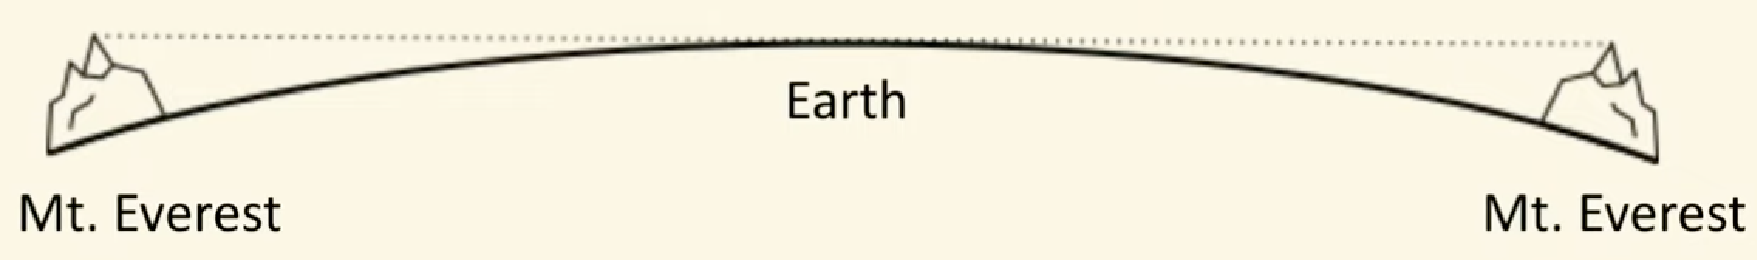
\includegraphics[width=0.9\textwidth]{lesson7/everest.pdf}
    \label{図: 1}
    \caption{実は光の直進性は欠点}
\end{figure}
地球は球なのでここから真裏の場所に直接行く方法はありません。なので、光も同様に直進して行くことは不可能でしょう。では今いる地点からどこまで見えるのでしょうか?これはエヴェレストなのですが、2つのエヴェレストがあるとして、これらはどの位離れているのでしょうか?

エヴェレストの高さは8848mでこの間の距離は\textbf{672km}になります。
そこで光の方向を選択・操作できればすごく役に立つでしょう。そのためにはどうすればいいでしょうか?
\subsection{Tyndallの実験}
これが1つ有名な実験なんですけれどもTyndallの実験(1870)です:
% Bucket, sun
\begin{figure}[H]
    \centering
    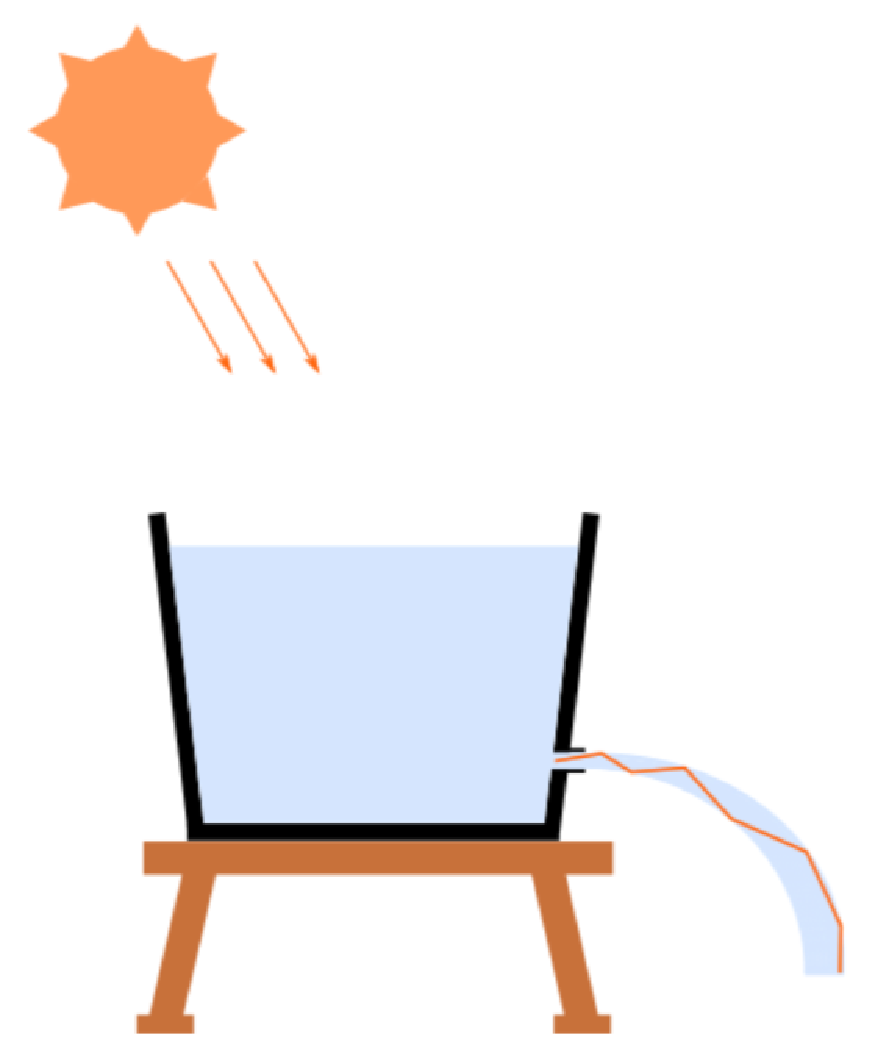
\includegraphics[width=0.5\textwidth]{lesson7/tyndall_cropped.pdf}
    \label{図: 1}
    \caption{Tyndallの実験}
\end{figure}

その実験はバケツを使ったのですが水が入ってて太陽の光が当たってて、下に穴が空いてました。穴から水が出てきたんですが水の中を太陽光が入っているところをイメージして下さい。太陽光が水に入って、下の穴から出て行ったわけです。\textbf{このアイデアを応用すれば、材料の中で光の進行方向を操作できるようになります}。この応用の中で 1番有名なものが\textbf{fiber optics(光ファイバー)です。}
\subsection{光ファイバーについて}

% Timeline
\begin{figure}[H]
    \centering
    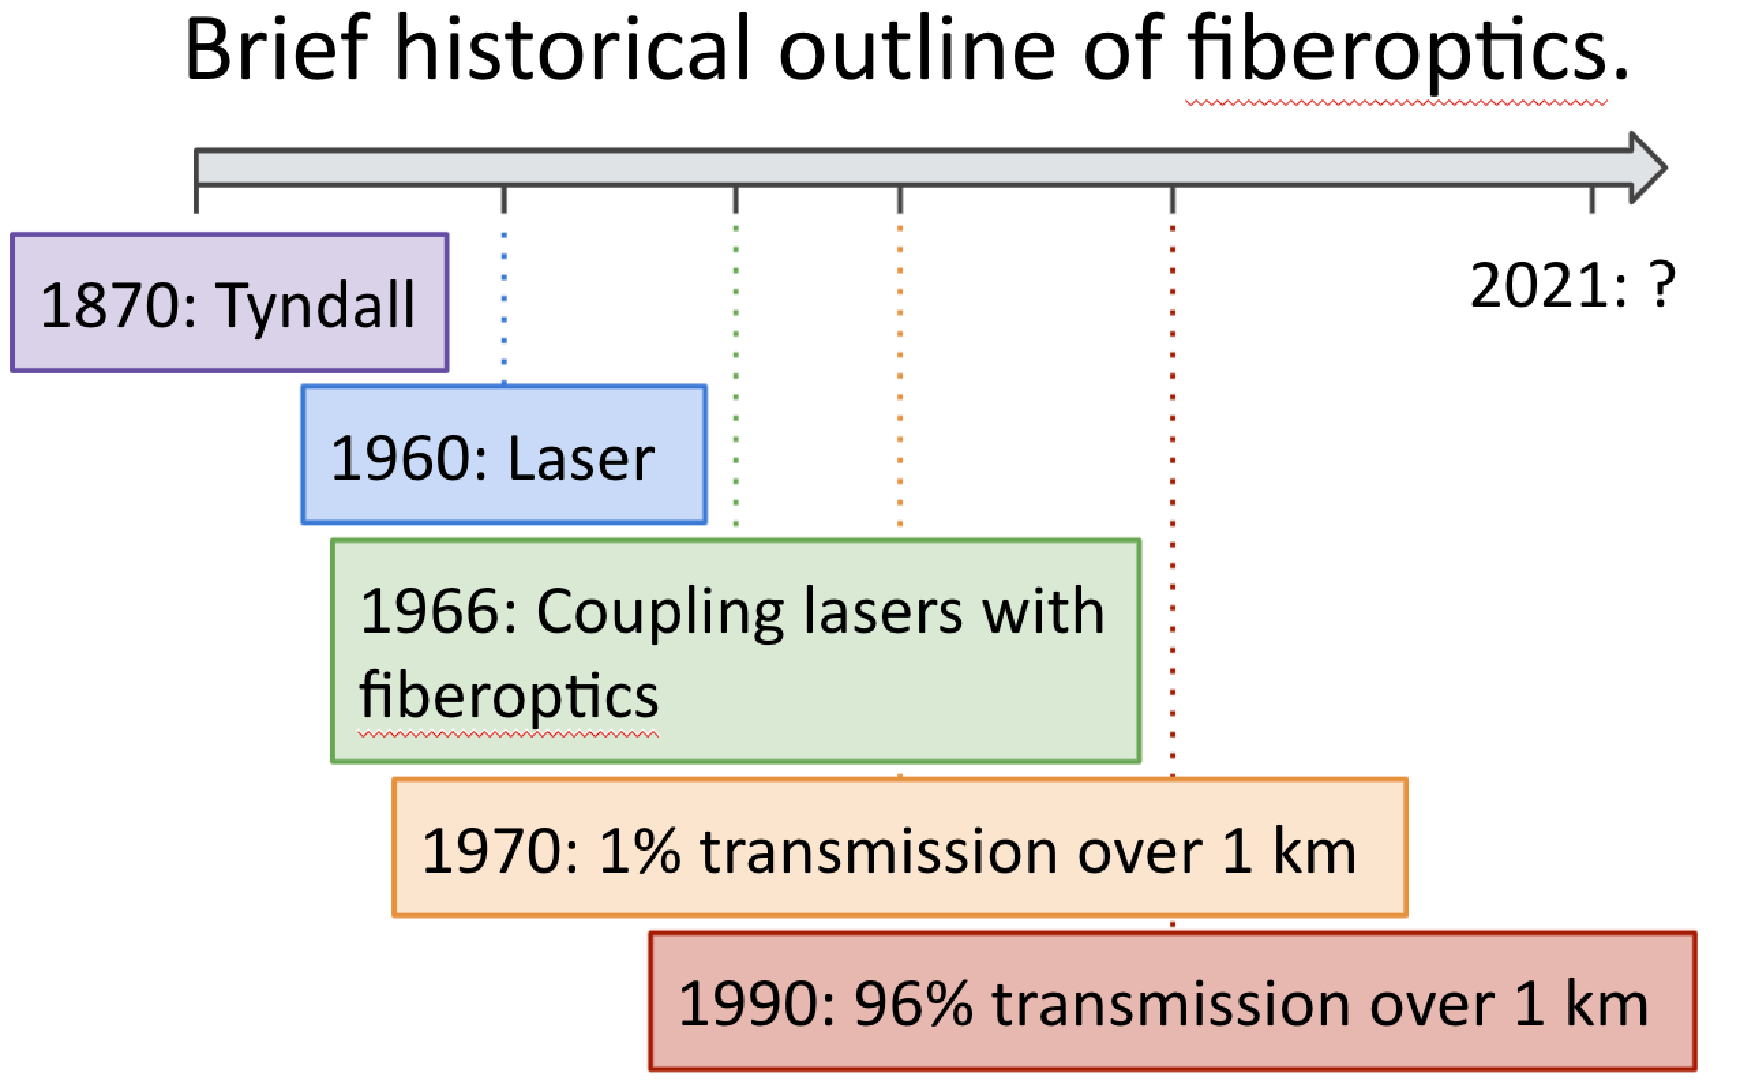
\includegraphics[width=0.9\textwidth]{lesson7/fiberoptics_timeline.pdf}
    \label{図: 1}
    \caption{光ファイバーの年表}
\end{figure}
Tyndallの実験はもう150年前のものですね。1960年にはレーザーが発明されて1966年僕の生まれた年なのですがレーザーと光ファイバーを合体させたものが誕生します。
1970年には1kmの光ファイバーの中で1\%の光が通るようになりました。その20年後にはその比率が1\%から96\%になりました。100\%にはなってないんですけれども素晴らしいでしょう。それだったらそれが1kmあたり96\%なので距離を伸ばすと段々比率は小さくなりますよね。でも素晴らしい技術の進化です。2021年にはどうなっているか、それは後で説明します。

% map
\begin{figure}[H]
    \centering
    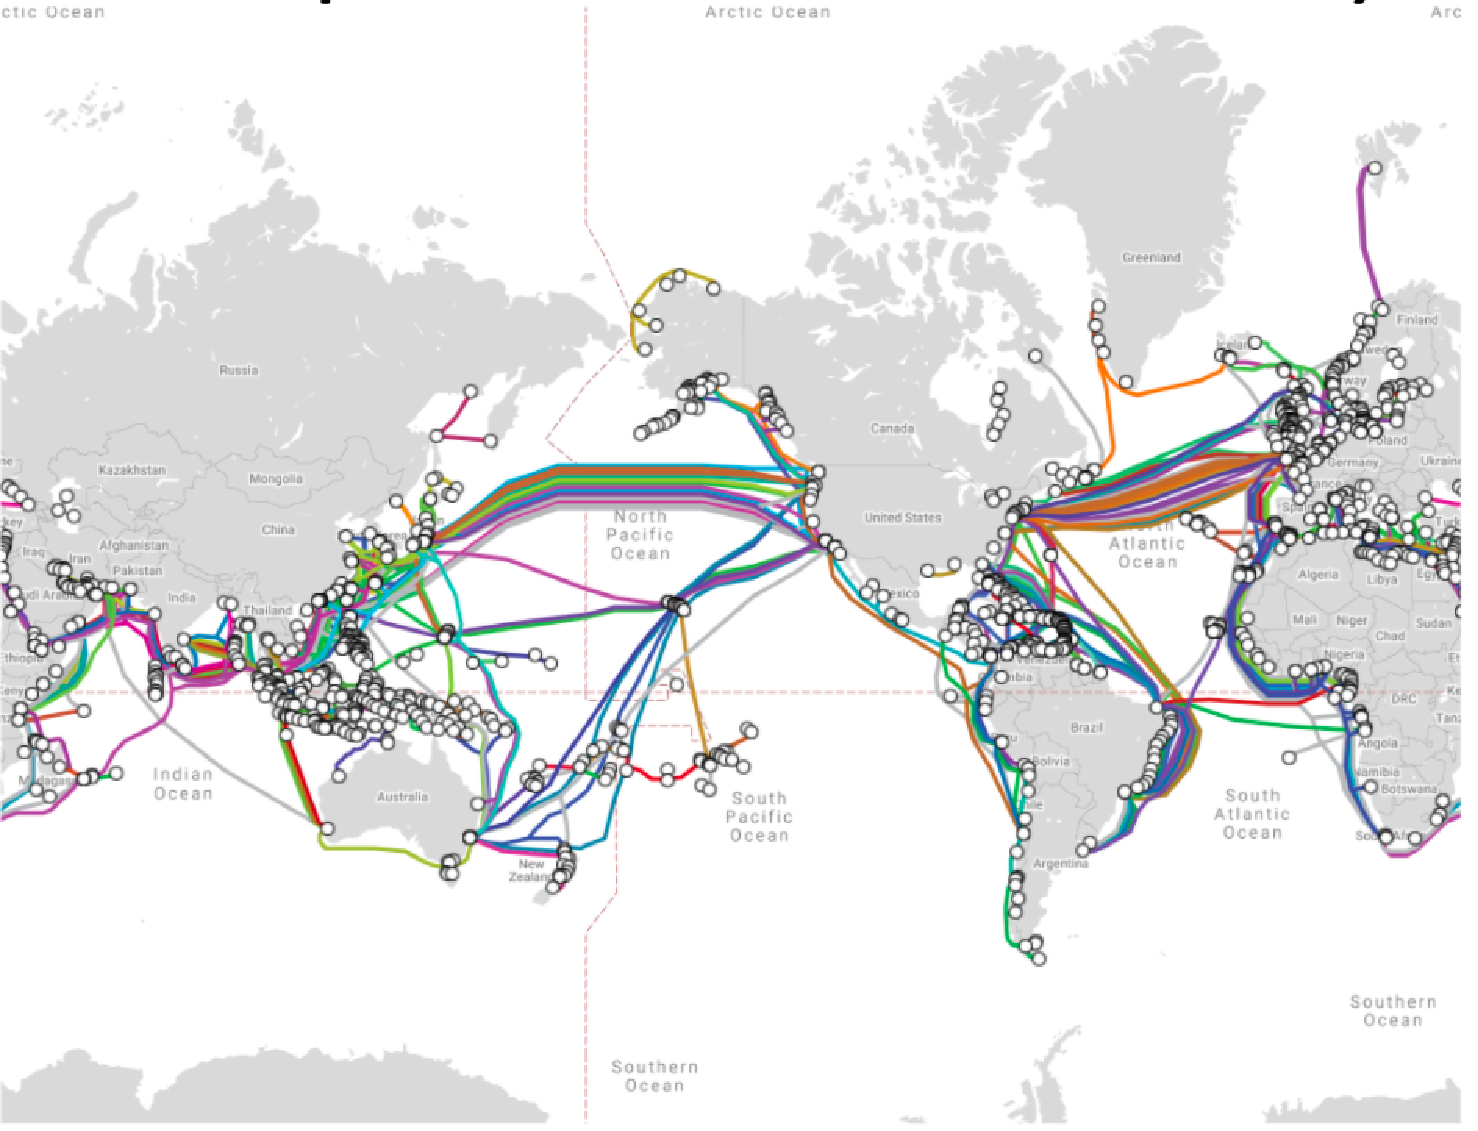
\includegraphics[width=0.9\textwidth]{lesson7/fibreoptics_map.pdf}
    \label{図: 1}
    \caption{全世界の光ファイバー}
\end{figure}
これは光ファイバーの全世界での使用例です。これはインターネットの通信とか
電話の通信とか色々使われているのですがこれぐらいのところがつながっているんですね。色んなところにこういう地図がネットには紹介されています。


で、光ファイバーについてちょっと説明したいと思います。まずは光が材料と材料の間のインターフェースに当たること\textbf{屈折}と\textbf{反射}について説明します。次に、どうやってファイバーの中に光を保存するのか。そして最後に光ファイバーのこと作る方法とかを説明します。


\section{境界面での光}
\section{全反射}
\section{光ファイバー}
% \section{クイズ}
